\documentclass{article}

\textwidth=6.5in
\textheight=8.5in
\voffset=-54pt
\oddsidemargin=0in
\evensidemargin=0in
\setlength{\parskip}{8pt}
\setlength{\parindent}{0pt}

\usepackage{amsmath, amssymb}
\usepackage{ifthen}

\usepackage[inline]{enumitem}
\setlist{topsep=0pt, parsep=8pt}

\usepackage[rgb,table]{xcolor}\convertcolorsUfalse
\usepackage{graphicx}

% change hyperref options
\PassOptionsToPackage{hyphens}{url}
\usepackage[bookmarks,colorlinks,linkcolor=black,citecolor=blue,pdfstartview=FitH,urlcolor=blue]{hyperref}
\hypersetup{pdfpagemode=UseNone}
\usepackage{bookmark}

\usepackage{graphicx}
\usepackage{multicol}
\usepackage{framed}
\usepackage{array}

\usepackage{icomma}

\usepackage{marginnote}
\usepackage[colorinlistoftodos]{todonotes}
\renewcommand{\marginpar}{\marginnote}

\usepackage{soul}
\usepackage[normalem]{ulem}

\usepackage{pgfplots}
\pgfplotsset{compat=1.18}  
\pgfplotscreateplotcyclelist{mycolor}{black, blue, red, green!70!black, magenta, purple, cyan, orange }  
\pgfplotsset{
  disabledatascaling,
  cycle list=tikzcolor, 
  axis lines=middle,
  every axis plot/.style={no marks, thick},
  every axis/.style={
    enlarge x limits=false,
    enlarge y limits=auto,
    xlabel style={at={(current axis.right of origin)},anchor=west},
    ylabel style={at={(current axis.above origin)},anchor=south},
    % extra x and y ticks for asymptotes
    extra x tick style={grid=major, grid style={dashed,black}},
    extra y tick style={grid=major, grid style={dashed,black}},
    /pgf/number format/1000 sep={},
  },    
  tick label style = {font=\footnotesize, fill=\currentbgcolor, inner sep=0pt},    
  xticklabel shift=1pt,    
  scaled ticks=false,
  scaled y ticks=false,
  unbounded coords=jump,
  samples=101,
  minor tick length=0,
  scatter/classes={
    open={mark=*,draw=black,fill=white, mark size=2, thin},
    closed={mark=*,draw=black,fill=black, mark size=2, thin}
  },
  width=3in,
}
\pgfplotsset{open/.style={only marks, mark=*, fill=white, thin, mark size=2}}
\pgfplotsset{closed/.style={only marks, mark=*, draw=black, fill=black,
    thin, mark size=2}}
\pgfplotsset{labeled/.style={nodes near coords, only marks, mark=*, draw=black, fill=black, thin, mark size=2, point meta=explicit symbolic}}

\usepackage{tikz}
\usetikzlibrary{
  matrix,%
  % enables the snake paths
  decorations.pathmorphing,%
  % enables bigger arrows
  decorations.markings,%
  decorations.pathreplacing,%
  decorations.text,%
  calc,%
  patterns,%
  shapes.geometric,%
  arrows,
  decorations.shapes,
  positioning,
  plotmarks,
  intersections
}
\tikzset{>=latex} % sets default arrow type in tikz
\tikzset{font=\normalsize}
\tikzset{mark size=1.5pt, mark options=thin}
\tikzset{pin distance=4pt,
  every pin edge/.style={<-, thin, shorten <= -2pt}}

\interfootnotelinepenalty=10000
\renewcommand{\thefootnote}{(\arabic{footnote})}

\usepackage{multirow, bigdelim}

% change to \usepackage[sols]{handout} to see solutions
\usepackage[]{handout}

\newcommand\iscurrentenumi[1]{%
  \ifthenelse{\equal{#1}{\theenumi}}{}{#1}}
\setenumerate[1]{ref=\#\arabic*}
\setenumerate[2]{ref=\protect\iscurrentenumi{\theenumi}(\alph*)}
\newcommand\enumiiprefix[2]{%
  \ifthenelse{{\equal{#1}{\theenumi}}\AND{\equal{#2}{(\alph{enumii})}}}{}{}%
  \ifthenelse{{\equal{#1}{\theenumi}}\AND{\NOT{\equal{#2}{(\alph{enumii})}}}}{#2}{}%
  \ifthenelse{\equal{#1}{\theenumi}}{}{#1#2}%
}
\setenumerate[3]{ref=\protect\enumiiprefix{\theenumi}{(\alph{enumii})}\roman*}

\newlength{\tipmargin}
\makeatletter

\newdimen\SOUL@dimen %new
\def\SOUL@ulunderline#1{{%
    \setbox\z@\hbox{#1}%
    % \dimen@=\wd\z@
    \SOUL@dimen=\wd\z@ %new
    \dimen@i=\SOUL@uloverlap
    \advance\SOUL@dimen2\dimen@i %\dimen@ exchanged too
    \rlap{%
      \null
      \kern-\dimen@i
      % \SOUL@ulcolor{\SOUL@ulleaders\hskip\dimen@}%
      \SOUL@ulcolor{\SOUL@ulleaders\hskip\SOUL@dimen}% new
    }%
    \unhcopy\z@
  }}

\renewenvironment{framed}{
  \setlength{\tipmargin}{\textwidth-\linewidth}
  \advance\@totalleftmargin-\tipmargin
  \def\FrameCommand{\hspace{\tipmargin}\fbox}%
  \advance\linewidth\tipmargin
  \MakeFramed {\advance\hsize-\width \FrameRestore}%
}
{\endMakeFramed}

\makeatother

\definecolor{purple}{rgb}{0.5,0,1.0}

\usepackage{fancyhdr}
\lhead{\textcolor{white}{This content is protected and may not be shared, uploaded, or distributed.}}
\rhead{}
\rfoot{\vspace*{\fill}\footnotesize\textcopyright{} \emph{Harvard Math Ma}}
\renewcommand{\headrulewidth}{0pt}
\pagestyle{fancy}
\begin{document}

\htitle{20. Finding Global Extrema}

\begin{problemonly}
  \begin{framed}

You should be able to:
    \begin{itemize}[topsep=0pt,partopsep=0pt,parsep=8pt,itemsep=0pt]
    \item Explain what the Extreme Value Theorem says.

    \item Determine whether a given function has global extrema on a given domain and, if so, find the global extrema.

    \end{itemize}
  \end{framed}
\end{problemonly}

\begin{enumerate}
\item 

  \note{This problem is meant to help students build intuition for the Extreme Value Theorem.} 

  Can you sketch an example of each of the following, or is it impossible?

  \probonly{\begin{multicols}{2}}
    \begin{enumerate}
    \item
      \begin{problem}[2in]
        A function that:
        \begin{itemize}[nosep]
        \item is continuous on $(-2, 2)$.
        \item has a global maximum value of 3 and no global minimum on $(-2, 2)$.\footnote{The phrase ``global maximum \uline{value} of 3'' means the $y$-value of the global maximum is 3, while the phrase ``global maximum \uline{at} 3'' means the $x$-value is 3.}
        \end{itemize}
      \end{problem}

      \begin{solution} 
        There are many possibilities; here's one. 
        \begin{center}
          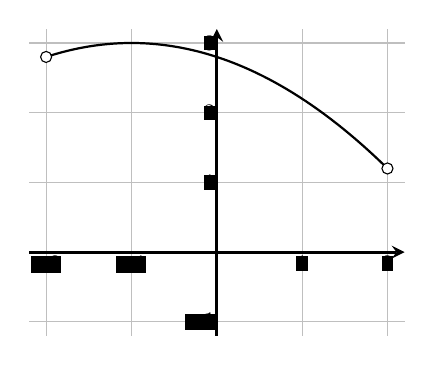
\begin{tikzpicture}
            \begin{axis}[ xmin=-2.2, xmax=2.2, ymin=-1.2, ymax=3.2, major tick length={0}, line width=1pt, axis lines=center, width=2.5 in, grid=major, restrict y to domain=-1:4 ]
              \addplot[open] coordinates{(-2,2.8)}; %
              \addplot[open] coordinates{(2,1.2)}; %
              \addplot [domain=-2:2] {-.2*(x+1)^2+3};
            \end{axis}
          \end{tikzpicture}
        \end{center}
      \end{solution}

    \item
      \begin{problem}[2in]
        A function that:
        \begin{itemize}[nosep]
        \item is defined on $[-2, 2]$.
        \item has a global minimum but no global maximum on $[-2, 2]$.
        \end{itemize}
      \end{problem}

      \begin{solution}
        Here's one possibility.
        \begin{center}
          \begin{tikzpicture}
            \begin{axis}[ xmin=-2.2, xmax=2.2, ymin=-1.2, ymax=3.2, width=2.5 in,
            grid=major]
              \addplot+[domain=-2:2] {x^2-1}; 
              \addplot[open] coordinates{(-2, 3) (2, 3)}; %
              \addplot[closed] coordinates{(-2, 1) (2, 1)}; %
            \end{axis}
          \end{tikzpicture}
        \end{center}
      \end{solution} 

    \item

      \note{This is an example where the hypotheses of the Extreme Value Theorem aren't satisfied, but the function still has both a global maximum and a global minimum on the domain.}

      \begin{problem}[2in]
        A function that:
        \begin{itemize}[nosep]
        \item is continuous on $(-2, 2)$.
        \item has both a global maximum and a global minimum on $(-2, 2)$.  
        \end{itemize}
      \end{problem}

      \begin{solution}
        Here's one possibility.
        \begin{center}
          \begin{tikzpicture}
            \begin{axis}[xmin=-2.2, xmax=2.2, ymin=-1.2, ymax=3.2, width=2.5 in,
            grid=major]
              \addplot+[domain=-2:2] {0.5*x^3-1.5*x+1}; 
              \addplot[open] coordinates{(-2, 0) (2, 2)}; %
            \end{axis}
          \end{tikzpicture}
        \end{center}
      \end{solution} 

    \item
      \begin{problem}[2in]
        A function that:
        \begin{itemize}[nosep]
        \item is continuous on $[-2, 2]$.
        \item does not have a global maximum on $[-2, 2]$. 
        \end{itemize}
      \end{problem}

      \begin{solution}
        This is impossible!
      \end{solution}

    \end{enumerate}
  \probonly{\end{multicols}}
  \pspace{\newpage}

\item 

  \note{Now, we'll state the Extreme Value Theorem.}

  \begin{problem}[\vfill]
    Under what conditions can we be sure that a function $f$ has a global maximum and a global minimum on a given domain?
  \end{problem}

  \begin{solution}
    If a function $f$ is continuous on a closed interval, then it must
    attain a global maximum and a global minimum on that interval.
  \end{solution}

\item  \label{critical-points-reasoning-set2}

  Suppose you've made the following sign chart for the derivative of a function $f(x)$. The function $f(x)$ is continuous and differentiable on $(-\infty, \infty)$.
  \begin{center}
    \begin{tikzpicture}
      \begin{axis}[axis y line=none, x axis line style={-}, xtick={0, 3, 5}, ymin=-2, height=1in, width=3.5in, clip=false]
        \addplot+[domain=-6:7.5, very thin]{0};
        \draw (-6, -1.5) node[right] {sign of $f'$};
        \draw (-1.25, -1.5) node{$+$};%
        \draw (1.5, -1.5) node{$-$};%
        \draw (4, -1.5) node{$+$};%
        \draw (6.25, -1.5) node{$-$};%
      \end{axis}
    \end{tikzpicture}    
  \end{center}

  \note{In all of these, it's worthwhile to ask:
    \begin{itemize}[nosep]
    \item If $f$ definitely has a global min / max, what additional work would you do to decide where that global min / max is? (For example, in (a), you would evaluate $f(0)$ and $f(5)$ and see which is higher.) 
    \item If $f$ might have a global min / max, what additional work would you to do to decide whether it does? 
    \end{itemize}
  }

  \begin{enumerate}
  \item

    \note{Here, it's also worth asking what the Extreme Value Theorem tells us about this situation, just to make sure students understand that it doesn't tell us anything.}

    \begin{problem}[\vfill]
      Does $f$ have a global maximum on $(-\infty, \infty)$? (Definitely yes, definitely no, or maybe?) If so, where could it be?
    \end{problem}

    \begin{solution}
      Yes, $f$ must have a global maximum at either $x = 0$ or $x = 5$.
    \end{solution}

  \item

    \begin{problem}[\vfill]
      Does $f(x)$ have a global minimum on $(-\infty, \infty)$? If so, where could it be?
    \end{problem}

    \begin{solution}
      There is not enough information to be sure. For example, it's possible that $\displaystyle \lim_{x \to \infty} f(x) = - \infty$, in which case $f$ certainly would not have a global minimum. However, it's also possible that $\displaystyle \lim_{x \to \infty} f(x)$ and $\displaystyle \lim_{x \to -\infty} f(x)$ both exist and that $x = 3$ is a global minimum point. Both possibilities are illustrated below:
      \begin{center}
        \begin{tikzpicture}
          \begin{axis}[xtick={3, 5}, ytick=\empty, enlargelimits=false,
            width=3in, ymax=600, clip=false] 
            \addplot+[domain=-2:7.5, samples=151]{500 - 90*x^2 + 32*x^3 -
              3*x^4}; 
          \end{axis}
        \end{tikzpicture}
        \hspace{0.5in}
        \begin{tikzpicture}
          \begin{axis}[xtick={3, 5}, ytick=\empty, enlargelimits=false,
            width=3in, ymin=0, extra y ticks={1}, extra y tick labels={},
            clip=false] 
            \addplot+[domain=-4:8]{2.718281828459045^(((-4.274856759437754 + x)*(-1.058476573895579 + x))/(1. + (-3.0676437038635322 + x)^2)^2)};
          \end{axis}
        \end{tikzpicture}
      \end{center}
    \end{solution}

  \item
    \begin{problem}[\vfill]
      Does $f$ have a global maximum on $[-2, 10]$? If so, where could it be?
    \end{problem}

    \begin{solution}
      Yes, $f$ must have a global maximum on $[-2, 10]$; it could be at $x = 0$ or $x = 5$.
    \end{solution}

  \item
    \begin{problem}[\vfill]
      Does $f$ have a global minimum on $[-2, 10]$? If so, where could it be?
    \end{problem}

    \begin{solution}
      Yes, $f$ must have a global minimum on $[-2, 10]$; it could be at $x = -2$, $x = 3$, or $x = 10$.
    \end{solution}

  \item
    \begin{problem}[\vfill\newpage]
      Does $f$ have a global minimum on $(-2, 10)$? If so, where could it be? 
    \end{problem}

    \begin{solution}
      We don't have enough information to tell. It's possible that the global minimum
      on $(-2, 10)$ is at $x=3$, but it's also possible that there is no global minimum
      due to the excluded endpoints. Both possibilities are illustrated below:
      \begin{center}
        \begin{tikzpicture}
          \begin{axis}[xtick={-1, 3, 7}, xticklabels={-2, 3, 10},
            ytick=\empty, enlargelimits=false, xmin=-2, xmax=7.5,
            width=3in, ymax=600, clip=false] 
            \addplot+[domain=-1:7, samples=151]{500 - 90*x^2 + 32*x^3 -
              3*x^4};
            \addplot[open] coordinates {(-1,375) (7, -137)};
          \end{axis}
        \end{tikzpicture}
        \hspace{0.5in}
        \begin{tikzpicture}
          \begin{axis}[xtick={-1, 3, 7}, xticklabels={-2, 3, 10},
          ytick=\empty, enlargelimits=false, xmin=-2, xmax=7.5,
            width=3in, ymin=0, clip=false] 
            \addplot+[domain=-1:7]{2.718281828459045^(((-4.274856759437754 + x)*(-1.058476573895579 + x))/(1. + (-3.0676437038635322 + x)^2)^2)};
            \addplot[open] coordinates {(-1, 1.0359) (7,1.0636)};
          \end{axis}
        \end{tikzpicture}
      \end{center}
    \end{solution}

  \end{enumerate}

\item  \label{global-extrema-strategy-1}

  \note{The strategy I want is:
    \begin{itemize}[nosep]
    \item Find the critical points, and plug each into $f$.
    \item Compare with end behavior (if the domain is a closed interval, plug the endpoints into $f$; if the domain is an open interval, take one-sided limits)
    \end{itemize}
  }

  \begin{problem}[1.5in]
    Summarize: What's a strategy for deciding whether a continuous function $f$ has a global min/max on a particular domain? (And, if it has one, how do you find where it is?)
  \end{problem}

  \begin{solution}
    Global extrema of continuous functions can only occur at critical
    points or endpoints. Therefore we should first find the critical points of
    $f$. Then we should plug each critical point into $f$ and get values.

    Next we need to determine end behavior. If there are any included endpoints, 
    then we should plug these into $f$ and get
    values. If there are excluded endpoints or if the domain is infinite, then
    we should take the appropriate one-sided limits of $f$ to determine the
    end behavior. 

    Finally, we compare all of the values and limits of $f$ that we found.
    If the greatest value/limit occurs at a critical point
    or an included endpoint, then $f$ has a global max there. If
    the greatest value/limit occurs at an excluded endpoint, then
    $f$ does not attain a global max on its domain. We repeat
    the same comparison for the global min, but we look for the
    least value/limit instead.
  \end{solution}

\begin{framed}
    The {\bf Extreme Value Theorem} guarantees the existence of a function's global extrema. Under what conditions does a function $f(x)$ definitely have a global max and a global min?
    \vspace{0.5in}
\end{framed}
\item 

  \note{Here, we'll carry out the strategy we just came up with.}    

  \begin{enumerate} 
  \item \label{optimization-can-1-abs-extrema-domain1}

    \begin{problem}[\vfill]
      Does $f(r) = 2 \pi r^2 + \dfrac{4000 \pi}{r}$ have a global maximum and global minimum on $[2, 20]$? If so, where? (Give the $r$-values at which the global minimum and global maximum occur.)
    \end{problem}

    \begin{solution}
      $f(r)$ is a continuous function defined on a closed interval. We know that it will have a global maximum and a global minimum because of the {Extreme Value Theorem}. First
      we need to find the critical points.
        $$f'(r) = 4 \pi r - \frac{4000 \pi} {r^2}$$
        $$ 0  =4 \pi r - \frac{4000 \pi} {r^2}$$
        $$ 4 \pi r = \frac{4000 \pi} {r^2}$$
        $$ r^3 = 1000$$ 
        $$ r =10$$ 
        So we need to calculate the values of $f$ at the critical point $10$ and 
        at the endpoints $2$ and $20$. 
        Note that the derivative does not exist at $0$, but we are only concerned about the 
        interval $[2,20]$
        \begin{center} 
          \begin{tabular} {c || c | c| c } 
            $x$ & 2 & 10 & 20  \\ 
            \hline 
            $f(x)$ &$2008 \pi$ &$600 \pi$  &$1000 \pi$ 
          \end{tabular} 
        \end{center} 
        From this table we see that, on $[2, 20]$,
        $(2,2008 \pi)$ is the global max and $(10, 600 \pi)$ is the global min. 
        This gives us enough information to sketch a graph. 
      \begin{center} 
        \begin{tikzpicture} [scale=.8]
          \begin{axis}[xtick={2,10,20}, ytick={1885, 3140, 6308}, 
            yticklabels={$600\pi$, $1000\pi$, $2008\pi$}]
            \addplot+[domain=2:20] [ultra thick,red] {2*3.14*x^2+4000*3.14/x};
            \addplot+[domain=0:1] [draw=none] {1800};
            \addplot[closed] []coordinates{(2,3.14*2008)};
            \addplot[closed] []coordinates{(10,3.14*600)};
            \addplot[closed] []coordinates{(20,3.14*1000)};
          \end{axis}
        \end{tikzpicture} 
      \end{center} 
    \end{solution}

  \item
    \begin{problem}[\nstretch{0.5}]
      Does $f$ have a global minimum and global maximum on $(0, \infty)$? If so, where?
    \end{problem}

    \begin{solution} 
       The \textcolor{blue}{Extreme Value Theorem} no longer applies since the domain we're
       considering is not a closed interval. The only critical point is at $10$. We know
       that the value of the function there is $600\pi$. Now we need to determine
       use one-sided limits of $f$ to determine the end behavior.

       \begin{itemize}
        \item $\displaystyle \lim_{r\to0^+} f(r) =
          \lim_{r\to0^+} \left(2 \pi r^2 + \frac{4000 \pi}{r}\right) = \infty. $
        \item $\displaystyle \lim_{r\to\infty} f(r) = 
          \lim_{r\to\infty} \left( 2 \pi r^2 + \frac{4000 \pi}{r}\right) = \infty$. 
       \end{itemize}
       
       From our analysis above we can see that, on $(0, \infty)$, $f$ attains
       a global minimum of $600\pi$ 
       at $10$, and $f$ does not attain a global maximum. 
    \end{solution} 

  \end{enumerate}

\item  

  \emph{A special case.} Maria is trying to determine whether a continuous function $f$ has a global maximum on $(1, 7]$. She's already determined that the only critical point of $f$ in $(1, 7]$ is $5$. 

  \begin{enumerate}
  \item

    \note{Here, Maria needs to check end behavior, which means comparing $\displaystyle \lim_{x \to 1^+} f(x)$ and $f(7)$.}

    \begin{problem}[\vfill]
      If Maria happens to know that 5 is a local minimum, what should she do next to finish deciding whether $f$ has a global maximum on $(1, 7]$? 
    \end{problem}

    \begin{solution}
      Maria needs to consider end behavior. Since the
      left endpoint is excluded, she should evaluate 
      $\lim\limits_{x \to 1^+} f(x)$. The right endpoint is included, so she should
      evaluate $f(7)$. Then she needs to compare the two values.
      If $f(7)$ is the larger value, then that is the global maximum on $(1, 7]$. 
      If $\lim\limits_{x \to 1+} f(x)$, then $f$ does not attain a global maximum on
      $(1, 7]$.
    \end{solution}

  \item

    \note{Here, Maria doesn't need to do any more! From what she's done already, we can be sure $f$ is increasing on $(1, 5)$ and decreasing on $(5, 7)$, so on $(1, 7]$, $f$ must have a global maximum at $x = 5$.}

    \begin{problem}[\vfill]
      If Maria instead happens to know that $5$ is a local maximum, what should she do next to finish deciding whether $f$ has a global maximum on $(1, 7]$? 
    \end{problem}

    \begin{solution}
      Since $5$ is a local maximum and it's the only critical point,
      $f$ is increasing on $(1, 5)$ and decreasing on $(5, 7)$.
      This means that Maria does not need to do anything
      else—she can say that the global maximum must be at $5$.
    \end{solution}

  \item \label{global-extrema-strategy-2}

    \note{If a function has only one critical point on the domain, and it's a local max, then it's also a global max (and similarly for min instead of max). So, if a function has only one critical point on the domain, we can use the First or Second Derivative Test to classify it. Of course, if it ends up being the wrong kind of local extremum (like a min when we're looking for a max), then we'll still need to test end behavior.}

    \begin{problem}[\vfill\newpage]
      Summarize: When can we use a strategy other than that in  \ref{global-extrema-strategy-1} to find whether / where a continuous function $f$ has a global min / max on a particular domain? 
    \end{problem}

    \begin{solution}
      If a function has only one critical point on a particular domain, we
      can use the First or Second Derivative Test to classify it.
      \begin{itemize}
        \item If the critical point is a local max, 
          then it is also the global max on that domain.
          We need to look at end behavior to determine whether there is a global min.
        \item If the critical point is a local min, 
          then it is the global min. 
          We need to look at end behavior to determine whether there is a global max.
        \item If the critical point is neither a min nor a max, then we need
          to look at end behavior to determine whether there is a global min/max.
          
      \end{itemize}
      
    \end{solution}

  \end{enumerate}

\item    

  \note{This ends up being the function and domain from \ref{optimization-can-1-abs-extrema-domain1}. Alternatively, since there's only one critical point, we can skip finding the domain and instead first try the First or Second Derivative Test.}  

  \begin{problem}[\vfill\newpage]
    A company sells canned tomatoes to restaurants. They want to pack the tomatoes in steel cans. Each can should have a volume of $2000 \pi$ cubic centimeters. The company's factory can only manufacture cans that are at least 5 cm tall and have a radius of at least 2 cm. In order to conserve resources, the company wants to minimize the amount of steel needed for each can. What dimensions should they make their cans?
  \end{problem}

  \begin{solution}
      Let's follow a strategy.
      \begin{enumerate}[label=\arabic*.] 
      \item \textbf{Name (and understand) some variables!  (If applicable,
          draw a picture to help with this.)} We are asked for dimensions of
        the can, so let's give names to these.  Let's call the radius of the
        can $r$ and the height of the can $h$.
      \item \textbf{Figure out what to optimize.}  We are asked to
        ``minimize the amount of steel needed for each can,'' so
        let's try to write an expression for this amount of steel.  We
        know we need steel for the sides of the can as well as the top
        and bottom.  The top and bottom are circles of radius $r$, so they
        each have area $\pi r^2$.  The sides have area $2 \pi r h$.  So, the
        total amount of steel (in square inches) is $2 \pi r^2 + 2 \pi r
        h$. 
      \item \textbf{Express the thing you're optimizing as a function of
          \textit{one} variable.}  Right now, we've expressed the total
        amount of steel as a function of both $r$ and $h$; we need to get
        it down to just one variable.  To do this, we need to \textbf{relate
          the variables $r$ and $h$}.  In this case, we can use the fact
        that the can has volume $2000 \pi$ cubic centimeters, which tells us
        that $\pi r^2 h = 2000 \pi$.\\
        We can either write $r$ in terms of $h$ or $h$ in terms of $r$.  It
        really makes no difference, but it looks like it's very slightly
        easier to solve for $h$ in terms of $r$, so let's do that.  Dividing
        the equation $\pi r^2 h = 2000 \pi$ by $\pi r^2$ gives $h =
        \frac{2000}{r^2}$.\\
        Therefore, the total amount of steel, as a function of just $r$,
        is $2 \pi r^2 + 2 \pi r \left( \frac{2000}{r^2} \right) = 2 \pi r^2 +
        \frac{4000 \pi}{r}$. 
      \item \textbf{Find the domain of the function we're maximizing.}  This
        is really important because the method we use for finding the
        absolute maximum or minimum of a function depends on whether the
        domain is a closed interval. The problem statement is specific about the lower bound for $r$: $$2 \leq r$$
        The upper bound for $r$ happens when $h$ is as small as possible. 
        $$ 2000 \pi = \pi r^2 (5)$$ 
        $$r^2 =400$$
        $$ r =20$$ 
        This means that the domain is $2 \leq r \leq 20$. This is exactly the
        same function and domain that we found the global extrema for in 
        \ref{optimization-can-1-abs-extrema-domain1}. We determined in that
        problem that the global min occurs when $r=10$.

        To fully answer the problem, we need to determine the value of $h$ that corresponds
        to this value of $r$. Since $h=\frac{2000}{r^2}$, when $r=10$, $h=20$. So the
        dimensions of the can that minimize the amount of steel needed are a radius of $10$
        cm and a height of $20$ cm.
      \end{enumerate}  
  \end{solution}

\item  \label{x/(x^2+1)}

  Let $f(x) = \dfrac{x}{x^2 + 1}$.
  \begin{enumerate}
  \item
    \begin{problem}[\vfill]
      Find all critical points of $f$ on $(-\infty, \infty)$. (Note: there are multiple approaches to differentiate this function - which do you prefer?)
    \end{problem}

    \begin{solution}
      $\displaystyle f'(x) = \frac{(x^2 + 1) 1 - x (2x)}{(x^2 + 1)^2} = \frac{1 - x^2}{(x^2 + 1)^2}$. $f'$ is never undefined, and it's 0 when $x = \boxed{\pm 1}$.
    \end{solution}

  \item
    \begin{problem}[\vfill]
      Classify each critical point as a local maximum, local minimum, or neither. Is it easier to do this using the First Derivative Test or the Second Derivative Test?
    \end{problem}

    \begin{solution}
      It looks like $f''$ will be a pain to calculate, so let's use the First Derivative Test to classify the critical points. Notice that the denominator of $f'$ is always positive; here are some example points we could test:
      \begin{align*}
        f'(-2) &= \frac{-3}{\text{positive}} < 0 \\
        f'(0) &= \frac{1}{\text{positive}} > 0 \\
        f'(2) &= \frac{-3}{\text{positive}} < 0 
      \end{align*}
      That gives the following sign chart for $f'$:
      \begin{center}
        \begin{tikzpicture}
          \begin{axis}[axis y line=none, x axis line style={-}, xtick={-1, 1}, xticklabels={$-1$, $1$}, ymin=-2, ymax=2, height=1.25in, width=3in]
            \addplot+[domain=-5:3, very thin]{0};
            \draw (axis cs: -5, -1.5) node[right] {sign of $f'$};
            \draw (axis cs: -5, 1) node[right] {$f$};
            \draw (axis cs: -2, -1.5) node{$-$};
            \draw[->, xshift=2pt] (axis cs: -2.8, 1.5) -- (axis cs: -1.2, 0.5);
            \draw (axis cs: 0, -1.5) node{$+$};
            \draw[->, xshift=2pt] (axis cs: -0.8, 0.5) -- (axis cs: 0.8, 1.5);
            \draw (axis cs: 2, -1.5) node{$-$};
            \draw[->, xshift=2pt] (axis cs: 1.2, 1.5) -- (axis cs: 2.8, 0.5);
            \draw[->, xshift=2pt] (axis cs: -1.2, 0.5) -- (axis cs: -0.8, 0.5);
            \draw[->, xshift=2pt] (axis cs: 0.8, 1.5) -- (axis cs: 1.2, 1.5);
          \end{axis}
        \end{tikzpicture}
      \end{center}
      So, $f$ has \fbox{a local minimum at $x = -1$ and a local maximum at $x = 1$}.
    \end{solution}

  \item
    \begin{problem}[\vfill]
      Does $f(x)$ have a global minimum on $(-\infty, \infty)$?  If so,
      where?  
    \end{problem}

    \begin{solution}
      From the sign chart alone, we cannot tell whether $f$ has a global minimum on $(-\infty, \infty)$. To be sure, we must compare $f(-1)$ and $\displaystyle \lim_{x \to \infty} f(x)$:
      \begin{align*}
        f(-1) &= - \frac{1}{2} \\
        \lim_{x \to \infty} f(x) &= 0
      \end{align*}
      Of these, $f(-1)$ is lower, so on $(-\infty, \infty)$, $f(x)$ has a global minimum \fbox{at $x = -1$}.
    \end{solution}

  \item
    \begin{problem}[\vfill]
      Does $f(x)$ have a global maximum on $(-\infty, \infty)$?  If so,
      where?  
    \end{problem}

    \begin{solution}
      The easiest way to answer this is to use symmetry: $f(-x) = \displaystyle \frac{-x}{(-x)^2 + 1} = - \frac{x}{x^2 + 1} = - f(x)$, so $f$ is an odd function. Since the interval $(-\infty, \infty)$ is symmetric about $0$ and we've already seen that the lowest point of $f$ on this interval is at $x = - 1$, the highest point must be \fbox{at $x = 1$}.
    \end{solution}

  \item
    \begin{problem}[\vfill]
      Does $f(x)$ have a global maximum on $[-0.5, 2]$?  If so, where?
    \end{problem}

    \begin{solution}
      Yes; from the sign chart, we can see it must happen \fbox{at $x = 1$}.
    \end{solution}

  \item
    \begin{problem}[\stretch{0.75}]
      Does $f(x)$ have a global minimum on $[-0.5, 2]$?  If so, where?
    \end{problem}

    \begin{solution}
      Yes. Based on the sign chart, we can see that it must happen at either
      $x=-0.5$ or at $x=2$, so we need to compare $f(-0.5)$ and $f(2)$. We can
      calculate that $f(-0.5) = -\frac{2}{5}$ and $f(2) = \frac{2}{5}$. Since $f(-0.5)$
      is lower, the global min happens at \fbox{$x=-0.5$}.
    \end{solution}

  \end{enumerate}

\end{enumerate}
\end{document}
